\documentclass[a4,12pt]{article}

\setlength{\oddsidemargin}{0pt} \setlength{\evensidemargin}{0pt}
\setlength{\textwidth}{\paperwidth} \addtolength{\textwidth}{-2truein}
\setlength{\textheight}{\paperheight}
\addtolength{\textheight}{-2truein} \setlength{\topmargin}{0pt}
\addtolength{\topmargin}{-\headheight}
\addtolength{\topmargin}{-\headsep}

\usepackage{graphicx,amsmath,amssymb}

\usepackage[UKenglish]{isodate}

\usepackage[pdftex,pdftitle={PHYS281 Report example},pdflang={en-GB}]{hyperref}

\usepackage[ignoreunlbld,norefs,nocites]{refcheck}

\usepackage[sort&compress,numbers]{natbib}
\bibliographystyle{apsrev4-2}

%\setcounter{tocdepth}{2}

\begin{document}

\title{Writing a scientific report: Example for PHYS281}

\author{Neil Drummond}

\maketitle

\begin{abstract}
This report example illustrates how figures generated using Matplotlib
can be incorporated into a report prepared using LaTeX\@.  In
addition, some general observations about the structure of a
scientific report are made.  The abstract should be brief and
to-the-point, and should be readable as a standalone piece of text. It
should not contain any citations unless they are fundamental to the
work as a whole, e.g., if the work is a critique of another paper.
The abstract should contain one or two sentences summarising the
conclusions.  This document may provide a useful template for a
PHYS281 report.
\end{abstract}

\tableofcontents

\section{Introduction}

Learning how to write a report is vitally important, whatever your
career plans, and it complements the skills in programming that you
learn in PHYS281.  Undergraduate physics coursework and exams often
consist of small, well-defined, quantitative problems that have short,
neat, pen-and-paper algebraic solutions.  This gives an almost
entirely misleading impression of what scientific work is actually
like.  Much of the work in solving real-world problems lies in asking
the right questions, deciding on an appropriate experimental,
theoretical or computational approach, implementing that approach,
obtaining (imperfect) results, understanding the significance and
limitations of those results and then writing up the work in a form
that others can build on.  In practice scientists spend a lot of time
reading and writing reports, papers and other documents.

The Introduction section of a report should motivate the work
described in the report and explain why the work is interesting or
useful.  Furthermore, the Introduction should provide context, such as
a discussion of previous works in the field or even (where relevant)
some historical background to the material being presented in the
report.  The Introduction should also explain what is going to be done
in the report.  The Introduction should generally be written in a
relatively accessible manner.

\section{Background theory}

Either in the Introduction or in a section near the start of the
report, you should describe the theoretical background.  In an actual
research paper, you can often assume that the readers have PhD-level
knowledge in the relevant field.  In a PHYS281 project, the level
should be appropriate for second-year undergraduate physics students.

Note that equations should be incorporated into sentences, punctuation
and all.  The line following an equation should not be indented,
unless it is a new paragraph.  For example, the Schr\"{o}dinger
equation for a single particle of mass $m$ moving in a potential
$U({\bf r})$ is
\begin{equation} -\frac{\hbar^2}{2m} \nabla^2 \psi + U({\bf r})\psi
= i\hbar \frac{\partial \psi}{\partial
  t}, \label{eq:schrodinger} \end{equation} where $\hbar$ is the
reduced Planck's constant, $\psi({\bf r},t)$ is the wave function and
${\bf r}$ and $t$ are position and time, respectively.

When you cite earlier works, you should ensure that you provide the
citation information needed to retrieve the article, i.e., the journal
name, the lead author name, the journal edition, the page/article
number and the year of publication.  You are welcome to include
additional information, such as the title of the paper.  It is usually
best to sort your bibliography in order of citation.  BibTeX can be
used to handle many of these issues automatically.  But even when you
use BibTeX, you should still cast a critical eye over your references,
to ensure that they are consistently formatted and contain all
citation information.

As an example of a citation, a widely used algorithm for sampling
multivariate probability distributions was first introduced for
sampling the Boltzmann distribution~\cite{Metropolis}.

\section{Validation of methodology~\label{sec:validation}}

There is freedom to choose appropriate section names and structure
here.  In a PHYS281 report, you will need a section or subsection in
which you present evidence that your program works.

\section{Results and discussion}

Figure~\ref{fig:example} shows a plot created with Matplotlib.  Every
figure should be called out from the text like this.  Likewise for
tables, as shown in Table~\ref{table:planets}.  On the other hand,
equations should be incorporated into sentences, as illustrated in
Eq.~(\ref{eq:schrodinger}).  When referring to material in a
different section, such as the material on validation in
Sec.~\ref{sec:validation}, LaTeX makes it easy to provide cross
references.

\begin{figure}[!htbp]
\centering
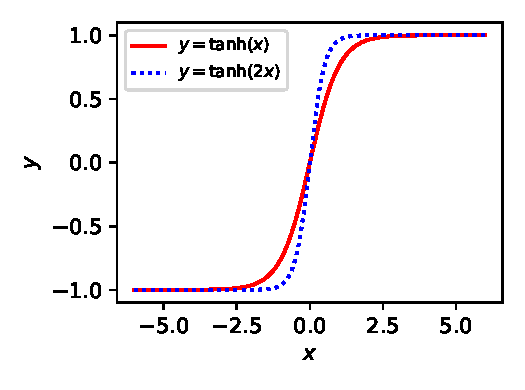
\includegraphics[clip,height=8cm]{tanh.pdf}
\caption{Plots of hyperbolic tangent functions, together with some
  example data.  Figure captions should be reasonably self-contained,
  such that it is not too difficult to work out what is going on
  without having read the rest of the report. (But there is no need to
  repeat introductory material or to redefine mathematical
  symbols.)~\label{fig:example}}
\end{figure}

\begin{table}[!htbp]
\centering

\caption{Masses and major exports between years 1947 and 2017 of some
  different planets. Note that numbers to be read by humans should use
  scientific notation, e.g., ``$6.02 \times 10^{23}$'' rather than
  ``6.02E23''.~\label{table:planets}}

\begin{tabular}{lcc}
\hline \hline

Planet & Mass (kg) & Major export \\

\hline

Earth & $5.972168 \times 10^{24}$ & Sitcoms, talk shows, etc. \\

Zibbleobbwob & $1.234 \times 10^{23}$ & Edible crinkleworms \\

\hline \hline
\end{tabular}

\end{table}

When including a figure, you should ensure that the font sizes of the
axis and tick labels and the legend are similar to (or even larger
than) the surrounding text in the report.

In your discussion, always be careful about value judgements.  If you
state that method X is better than method Y then you need to provide
(i) a clear definition of your criterion for being ``better'' and (ii)
evidence (or citation of evidence) that method X fulfils your
criterion more closely than method Y\@.

To prepare the PHYS281 report you do not need to use LaTeX, although
LaTeX makes it relatively easy to format equations, insert cross
references, manage citations and produce publication-quality
documents.  You are welcome to use whatever editing software (e.g.,
Visual Studio Code) or online editors (e.g.,
\href{https://www.overleaf.com/}{Overleaf}) that you like.

\section{Conclusions}

Your report should contain a Conclusions section, providing your
take-home messages.  Good reports have conclusions; mediocre reports
have summaries.

\appendix

\section{Additional information}

You are welcome to provide appendices to your report.  Realistically
the marker is not going to read your appendices, so they are just
there for your own satisfaction.

Reference~\cite{Perdew} is a remarkable example of a paper in which
Appendix C contains the most important material in the work.

\bibliography{my_bibliography}

\end{document}
